\documentclass[11pt]{article}
\usepackage[T1]{fontenc}
\usepackage[utf8]{inputenc}
\usepackage{lmodern}
\usepackage{amsmath,amssymb,amsthm}
\usepackage[letterpaper,margin=1.1in]{geometry}
\usepackage{microtype}
\usepackage{tikz}
\usetikzlibrary{decorations.markings}
\usepackage[colorlinks=true,linkcolor=blue!45!black,citecolor=blue!45!black,urlcolor=blue!45!black]{hyperref}

\newtheorem{theorem}{Theorem}[section]
\newtheorem{lemma}[theorem]{Lemma}
\newtheorem{proposition}[theorem]{Proposition}
\newtheorem{corollary}[theorem]{Corollary}
\theoremstyle{definition}
\newtheorem{problem}[theorem]{Problem}
\theoremstyle{remark}
\newtheorem{remark}[theorem]{Remark}

\newcommand{\Z}{\mathcal{Z}}
\newcommand{\X}{\mathcal{X}}
\newcommand{\PP}{\mathbb{P}}
\newcommand{\EE}{\mathbb{E}}
\newcommand{\comp}{\operatorname{comp}}
\newcommand{\dist}{\operatorname{dist}}
\newcommand{\tr}{\operatorname{tr}}
\newcommand{\lgs}{\log^{*}}
\newcommand{\lgk}[1]{\log^{(#1)}}
\newcommand{\sm}{\setminus}
\newcommand{\half}{\tfrac12}
\newcommand{\cO}{\mathcal{O}}

\title{The minimum number of edges in a pancyclic graph\\ and the number of cycles in a graph}
\author{}
\date{Draft of 10 November 2026}

\begin{document}
\maketitle

\begin{abstract}
Let $n+h(n)$ be the least number of edges of a pancyclic graph on $n$ vertices, that is, of a graph
that contains a cycle of every length from $3$ to $n$. KNT recently proved that
$h(n)=\log_2 n+\lgs n+O(1)$, as Erd\H{o}s had asked. The proof rests on one estimate: if a small union
of cycles $W$ is removed from a connected graph of large cycle rank, then a uniformly random even
subgraph, restricted to the remaining edges, is a forest with probability at most $\half+o(1)$.

We give a compact account of the theorem, organised around this estimate and a single counting lemma,
and record what else the two of them give. First, a graph of cycle rank $r$ has at most
$(\half+o(1))2^{r}$ cycles. This answers, asymptotically, a question of Entringer and Slater from 1981;
it was known for planar graphs and for graphs of average degree slightly above $4$, while for cubic
graphs the best bound was $\frac{15}{16}2^{r}$. Second, we describe the regime in which the counting
lemma loses nothing: it cannot last for more than $|V(W)|+3$ ranks beyond $W$, and a two-terminal graph
that carries $k$ binary digits of path lengths without loss has no path between its terminals with fewer
than $k$ edges. These elementary facts account for the shape of the extremal construction and show where the
iterated logarithm comes from.
\end{abstract}

\section{Introduction}\label{sec:intro}

A graph on $n$ vertices is \emph{pancyclic} if it contains a cycle of every length $3,4,\dots,n$.
Let $n+h(n)$ be the least number of edges of a pancyclic graph on $n$ vertices. Throughout, $\log$ is
the binary logarithm, $\lgk{j}$ is its $j$-fold iterate, $\lgs x$ is the least $j\ge0$ with
$\lgk{j}x\le1$, and $\ln$ is the natural logarithm. Graphs are finite and, unless we say otherwise,
simple.

\begin{theorem}[KNT~\cite{KNT}]\label{thm:main}
There is an absolute constant $A$ such that, for every $n\ge3$,
\[
  \log n+\lgs n-A\;\le\;h(n)\;\le\;\lfloor\log n\rfloor+\lgs n+1 .
\]
\end{theorem}

Bondy~\cite{Bondy} stated without proof that $\log(n-1)-1\le h(n)\le\log n+\lgs n+O(1)$. The lower
bound is a count: a connected graph with $n+h$ edges has at most $2^{h+1}-1$ cycles, and a pancyclic
graph needs $n-2$ of them. A proof of it was written down by Griffin~\cite{Griffin}, and the first
published proof of the upper bound appears to be the one in the book of George, Khodkar and
Wallis~\cite[\S4.5]{GKW}; see~\cite{Bloom}. Erd\H{o}s believed that the upper bound is closer to the truth, but could
not even show that $h(n)-\log n\to\infty$; this is Problem~\#1016 in Bloom's collection of Erd\H{o}s problems.
Theorem~\ref{thm:main} confirms his belief.

\paragraph{Two ingredients.}
For a graph $G$ let $\Z(G)$ be its cycle space over $\mathbb{F}_2$: the set of \emph{even subgraphs},
that is, of edge sets that meet every vertex an even number of times, with symmetric difference as
addition. Its dimension is the \emph{cycle rank} $\beta(G)=|E(G)|-|V(G)|+\comp(G)$, where $\comp$
counts components. A \emph{cycle} is a connected $2$-regular subgraph, and we do not distinguish
between a subgraph without isolated vertices and its edge set.

The count above uses only that the cycles of a graph are distinct elements of $\Z(G)$. To use that
their lengths fill an interval, fix a subgraph $W\subseteq G$ and sort the even subgraphs $\xi$ of $G$
by their \emph{outside part} $\xi\sm E(W)$. If $\beta(G)=r$, $\beta(W)=t$ and $W$ has $m$ edges, there
are $2^{r-t}$ possible outside parts, and cycles with the same outside part differ only inside $W$, so
they have at most $m$ different lengths. Hence $G$ has cycles of at most $m\,2^{r-t}$ lengths. When
$W$ is a union of cycles of lengths $3,4,5,\dots$ this can be nearly attained, as long as $r$ is not
much larger than $t$. The theorem that drives everything says that it is off by a factor of two once
$r$ is large: the outside part of a cycle that meets $W$ is a forest, and only half of the outside
parts are forests.

\begin{theorem}[Forest estimate, KNT~\cite{KNT}]\label{thm:forest}
There is $r_0$ such that the following holds for all $r\ge r_0$. Let $G$ be a connected simple graph
with $\beta(G)=r$, and let $W\subseteq G$ be a nonempty union of cycles with at most $\sqrt r$ edges
and at most $(\log r)/100$ components. If $\xi$ is a uniformly random element of $\Z(G)$, then
\begin{equation}\label{eq:forest}
  \PP\bigl(\xi\sm E(W)\text{ is a forest}\bigr)\;\le\;\frac12+\frac{20}{\lgk{3}r}.
\end{equation}
\end{theorem}

The constant $\half$ is best possible (Remark~\ref{rem:twoports}). Section~\ref{sec:lower} derives the
lower bound of Theorem~\ref{thm:main}: a witness $W$ of rank about $2R$ that contains the short cycles
has few edges, so~\eqref{eq:forest} applies to every graph of rank $2^{256R}$, and the quantity
$\max(\text{number of lengths})/2^{\text{rank}}$ halves each time the rank passes one exponential
level. Section~\ref{sec:upper} gives the construction and Section~\ref{sec:forest} proves
Theorem~\ref{thm:forest}.

\paragraph{The number of cycles.}
Let $\psi(r)$ be the largest number of cycles in a graph of cycle rank $r$. Entringer and
Slater~\cite{ES} observed that $\psi(r)\le2^{r}-1$, that the maximum is attained by cubic graphs and
that $\psi(r)>2^{r-1}$, and they asked whether $2^{r-1}$ is essentially the truth; this is usually
quoted as the conjecture $\psi(r)\sim2^{r-1}$. Aldred and Thomassen~\cite{AT} proved
$\psi(r)\le\frac{15}{16}2^{r}$, and $2^{r-1}+o(2^{r-1})$ for planar graphs. Alahmadi, Aldred, dela
Cruz, Sol\'e and Thomassen~\cite{AACST} showed that a graph with $p$ vertices and $q>2p+3\log(3p)$
edges has at most $2^{q-p}$ cycles. This left the sparse graphs, and in particular the cubic ones, for
which $\frac{15}{16}2^{r}$ remained the best bound that we are aware of~\cite{HK}. The forest estimate
closes this gap.

\begin{theorem}\label{thm:cycles}
For all sufficiently large $r$,
\[
  \psi(r)\;\le\;\Bigl(\frac12+\frac{21}{\lgk{3}r}\Bigr)2^{r}.
\]
In particular $\psi(r)\sim2^{r-1}$.
\end{theorem}

\paragraph{Exact counting.}
The factor $\half$ is forced only when the rank is large. Our second complement describes the opposite
regime, in which nothing is lost at all.

\begin{theorem}\label{thm:exact}
\textup{(a)} Let $N$ be a connected graph and let $s\ne t$ be two of its vertices. Then $N$ has at
most $2^{\beta(N)}$ paths from $s$ to $t$. If it has exactly $2^{\beta(N)}$, then each of these paths
has at least $\beta(N)$ edges, and deleting the edges of any one of them leaves a forest.

\textup{(b)} Let $G$ be a connected graph and let $W\subseteq G$ be a subgraph that contains a cycle.
If every coset of $\Z(W)$ in $\Z(G)$ contains a cycle, then $G-E(W)$ has no two edge-disjoint cycles,
and $\beta(G)\le\beta(W)+|V(W)|+3$.
\end{theorem}

Part~(b) says that the count described above can be exact for at most $|V(W)|+3$ ranks beyond $W$.
Part~(a) says that a gadget which turns $k$ units of rank into $2^{k}$ path lengths, like the necklace
in the construction of Section~\ref{sec:upper}, has no path between its terminals with fewer than $k$ edges. The cycles
through it are therefore long, the short cycle lengths have to come from a second, exponentially
smaller gadget, and so on: this is where the iterated logarithm comes from in the construction. The
lower bound of Theorem~\ref{thm:main} says that allowing losses does not help by more than a constant.
Section~\ref{sec:exact} also contains a stability statement of the same elementary kind
(Proposition~\ref{prop:defect}).

\paragraph{What is new.}
Theorems~\ref{thm:main} and~\ref{thm:forest} and the strategy of their proofs are due to
KNT~\cite{KNT}, whose argument has been formalised in Lean~4. Sections~\ref{sec:lower},
\ref{sec:upper} and~\ref{sec:forest} follow~\cite{KNT}. The changes there are expository: one counting
lemma (Lemma~\ref{lem:count}) serves both applications, the link formula is proved without
contractions, and the two facts needed about the non-backtracking matrix are derived directly.
Theorems~\ref{thm:cycles} and~\ref{thm:exact} and Proposition~\ref{prop:defect} are new as far as we
know. They have not been formalised; as a check, the elementary statements of
Sections~\ref{sec:count}, \ref{sec:upper} and~\ref{sec:exact} and the lemmas of
Section~\ref{sec:forest} on links and on the non-backtracking matrix were tested by computer on
small graphs.

\section{Counting by cosets}\label{sec:count}

Let $W$ be a subgraph of a graph $G$, and put $r=\beta(G)$, $t=\beta(W)$ and $m=|E(W)|$. The map
$\xi\mapsto\xi\sm E(W)$ is linear on $\Z(G)$ with kernel $\Z(W)$. We call the elements of its image
$\X=\X(G,W)$ \emph{words}. There are $2^{r-t}$ words, each word is the outside part of exactly $2^{t}$
even subgraphs, and if $\xi$ is uniform on $\Z(G)$ then $\xi\sm E(W)$ is uniform on $\X$. Let
\[
  p(G,W)=\PP\bigl(\xi\sm E(W)\text{ is a forest}\bigr)
\]
be the proportion of words that are forests.

\begin{lemma}[Counting lemma]\label{lem:count}
With this notation and $p=p(G,W)$,
\begin{enumerate}
\item[\textup{(a)}] $G$ has at most $2^{r}p+2^{r-t}(1-p)\le2^{r}\bigl(p+2^{-t}\bigr)$ cycles;
\item[\textup{(b)}] the cycles of $G$ have at most $2^{r-t}\bigl(pm+1-p\bigr)$ different lengths.
\end{enumerate}
\end{lemma}

\begin{proof}
Let $C$ be a cycle of $G$ with word $x=C\sm E(W)$. If $x$ is not a forest, it contains a cycle, and
since $x\subseteq C$ this forces $C=x$; so a word that is not a forest is the outside part of at most
one cycle. If $x$ is a forest, it is the outside part of at most $2^{t}$ cycles $C$, and
$C\cap E(W)\ne\emptyset$ for each of them, because $C\ne x$ when $x\ne\emptyset$ and $C\subseteq W$
when $x=\emptyset$. So their lengths $|x|+|C\cap E(W)|$ take at most $m$ values. Now sum over the
$p\,2^{r-t}$ words that are forests and the $(1-p)2^{r-t}$ words that are not.
\end{proof}

\begin{remark}[Two points of attachment]\label{rem:twoports}
Suppose that $G=W\cup N$, where $W$ and $N$ are connected, have no common edge, and have exactly two
common vertices $s$ and $t$. An \emph{$\{s,t\}$-join} of $N$ is an edge set in which $s$ and $t$ have
odd degree and all other vertices have even degree. The words are the $2^{\beta(N)}$ even subgraphs of
$N$ and the $2^{\beta(N)}$ joins of $N$, and a nonempty even subgraph is not a forest. Hence
\[
  p(G,W)\;\le\;\tfrac12+2^{-(r-t)} .
\]
So~\eqref{eq:forest} is trivial, and holds without the error term, for a subgraph attached at two
vertices. Equality holds when every join of $N$ is a path, for instance when $N$ is a chain of $k$
four-cycles joined at opposite vertices and $s,t$ are its two ends. With $W$ a triangle this example
also shows that the constant $\half$ in~\eqref{eq:forest} cannot be lowered.
\end{remark}

\section{The lower bound}\label{sec:lower}

For an integer $R\ge1$ let $\Phi(R)$ be the supremum of $(L-2)\,2^{-\beta(G)}$ over all simple graphs
$G$ with $\beta(G)\ge R$ and all integers $L\ge2$ such that $G$ contains a cycle of each length
$3,\dots,L$. Since a graph of rank $\beta$ has at most $2^{\beta}-1$ cycles, $\Phi(R)\le1$, and
$\Phi$ is non-increasing.

\begin{lemma}[Witness]\label{lem:witness}
Let $R\ge1$ and $\varphi=\Phi(R)$, and let $G$ contain a cycle of each length $3,\dots,L$, where
$L\ge2^{2R}$. Then $G$ has a subgraph $W$ that is a union of at most $2R$ cycles, with
$\beta(W)\ge2R$ and $|E(W)|\le\varphi\,2^{2R}+2^{R}+5R$.
\end{lemma}

\begin{proof}
Put $W_0=\emptyset$ and $W_{i+1}=W_i\cup C_i$, where $C_i$ is a cycle of $G$ whose length $\ell_i$ is
the least integer $\ge3$ that is not the length of a cycle of $W_i$; stop as soon as the rank is at
least $2R$. Let $s=\beta(W_i)<2R$. The graph $W_i$ contains cycles of the $\ell_i-3$ lengths
$3,\dots,\ell_i-1$. Therefore $\ell_i-3\le2^{s}-1$, which gives $\ell_i\le2^{2R-1}+2\le L$, so that
$C_i$ exists; and $\ell_i-3\le\varphi\,2^{s}$ if $s\ge R$, by the definition of $\Phi$. As $C_i$ is
not a subgraph of $W_i$, the rank increases at every step. So there are at most $2R$ steps, their
ranks $s$ are distinct, and
\[
  |E(W)|\;\le\;\sum_i\ell_i\;\le\;\sum_{s=0}^{R-1}\bigl(2^{s}+2\bigr)+\sum_{s=R}^{2R-1}\bigl(\varphi\,2^{s}+3\bigr)
  \;\le\;\varphi\,2^{2R}+2^{R}+5R .\qedhere
\]
\end{proof}

\begin{proposition}[Near-halving]\label{prop:halving}
For every sufficiently large integer $R$,
\[
  \Phi\bigl(2^{256R}\bigr)\;\le\;\Bigl(\frac12+\frac{20}{\lgk{2}R}\Bigr)\Phi(R)+2^{2-R}.
\]
\end{proposition}

\begin{proof}
Let $G$ be a simple graph of rank $r\ge2^{256R}$ with a cycle of each length $3,\dots,L$. Identifying
a vertex of one component with a vertex of another changes neither the rank nor the set of cycles, so
we may assume that $G$ is connected. If $L<2^{2R}$ then $(L-2)2^{-r}<2^{2-R}$. Otherwise let $W$ be
as in Lemma~\ref{lem:witness}, with $m$ edges and rank $t\ge2R$. Then $m\le2^{2R+1}\le\sqrt r$ and
$\comp(W)\le2R\le(\log r)/100$, so Theorem~\ref{thm:forest} gives
$p(G,W)\le\half+20/\lgk3 r\le\half+\delta$ with $\delta=20/\lgk2R$; here we used
$\lgk3 r\ge\log(8+\log R)\ge\lgk2 R$. By Lemma~\ref{lem:count}(b),
\[
  \frac{L-2}{2^{r}}\;\le\;\frac{pm+1}{2^{t}}
  \;\le\;\Bigl(\frac12+\delta\Bigr)\bigl(\varphi+2^{-R}+5R\,2^{-2R}\bigr)+2^{-2R}
  \;\le\;\Bigl(\frac12+\delta\Bigr)\varphi+2^{2-R}.\qedhere
\]
\end{proof}

\begin{corollary}\label{cor:phi}
There is a constant $c$ such that $\Phi(r)\le c\,2^{-\lgs r}$ for all $r\ge1$.
\end{corollary}

\begin{proof}
Fix $R_0\ge2^{18}$ so large that Proposition~\ref{prop:halving} holds for all $R\ge R_0$, and let
$R_{j+1}=2^{256R_j}$ and $\delta_j=20/\lgk2R_j$. For $j\ge2$ we have $\lgk2R_j=8+256R_{j-2}$, so
$\sum_j\delta_j<\infty$; also $\sum_j2^{\,j-R_j}<\infty$. The numbers $a_j=2^{j}\Phi(R_j)$ satisfy
$a_{j+1}\le(1+2\delta_j)a_j+2^{\,j+3-R_j}$ and are therefore bounded, say $\Phi(R_j)\le c_1 2^{-j}$.

Next, let $U_0=R_0^2$ and $U_{j+1}=2^{U_j}$. Then $R_j\le\sqrt{U_j}$ for all $j$: inductively,
$R_{j+1}=2^{256R_j}\le2^{256\sqrt{U_j}}\le2^{U_j/2}$ because $\sqrt{U_j}\ge512$. Hence
$\lgs R_j\le\lgs U_j=j+\lgs U_0$.

Finally let $r\ge R_0$ and let $j$ be largest with $R_j\le r$. Then
$\Phi(r)\le\Phi(R_j)\le c_12^{-j}$ and $\lgs r\le\lgs R_{j+1}\le j+1+\lgs U_0$. For $r<R_0$ use
$\Phi\le1$.
\end{proof}

\begin{proof}[Proof of the lower bound in Theorem~\ref{thm:main}]
Let $G$ be a pancyclic graph with $n$ vertices and $n+h$ edges. It is connected, so its rank is
$r=h+1$, and by Corollary~\ref{cor:phi}
\[
  n-2\;\le\;\Phi(r)\,2^{r}\;\le\;c\,2^{\,r-\lgs r}.
\]
The trivial bound $n-2\le2^{r}-1$ gives $n\le2^{r+1}\le2^{2^{r}}$, hence $\lgs n\le\lgs r+2$. Taking
logarithms, $h=r-1\ge\log(n-2)+\lgs r-\log c-1\ge\log n+\lgs n-\log c-5$.
\end{proof}

\section{The construction}\label{sec:upper}

\begin{proposition}\label{prop:upper}
For every $n\ge3$ there is a pancyclic graph with $n$ vertices and at most
$n+\lfloor\log n\rfloor+\lgs n+1$ edges.
\end{proposition}

\begin{proof}
For $3\le n\le6$ take a cycle $u_0u_1\cdots u_{n-1}$, with the chord $u_0u_2$ if $n\ge4$ and also
the chord $u_0u_3$ if $n=6$.

Let $n\ge7$, and let $k\ge2$ be the largest integer with $2^{k}+k+1\le n$, so that
$n\le2^{k+1}+k+1$. Let $H$ be a cycle of length $n$ and let $Q\subseteq H$ be a path composed of
consecutive segments $Q_0,\dots,Q_{k-1}$, where $Q_i$ has $2^{i}+1$ edges and joins $v_i$ to
$v_{i+1}$. Thus $Q$ has $2^{k}+k-1\le n-2$ edges. Add the chords $e_i=v_iv_{i+1}$ for $0\le i<k$,
and let $N_j$, the \emph{necklace with $j$ beads}, be the union of $Q_0,\dots,Q_{j-1}$ and
$e_0,\dots,e_{j-1}$ (Figure~\ref{fig:necklace}).

A path from $v_0$ to $v_j$ in $N_j$ uses either $Q_i$ or $e_i$ for each $i<j$, and replacing $Q_i$ by
$e_i$ shortens it by $2^{i}$. So $N_j$ has $2^{j}$ such paths, exactly one of each length from $j$ to
$2^{j}+j-1$. Consequently a chord $f_j=v_0v_j$ with $j\ge2$ creates cycles of all lengths in
$I_j=[\,j+1,\ 2^{j}+j\,]$, and the path $H-Q$ together with $N_k$ contains cycles of all lengths in
$[\,n-2^{k}+1,\ n\,]$.

Let $j_0=k$ and $j_{i+1}=\lceil\log j_i\rceil$ as long as $j_i>2$; this sequence decreases and ends
with some $j_q=2$. Add the chords $f_{j_0},\dots,f_{j_q}$. Since $2^{j_{i+1}}\ge j_i$, the intervals
$I_{j_{i+1}}$ and $I_{j_i}$ overlap or are adjacent, and $I_2=[3,6]$; so we get all lengths in
$[3,\ 2^{k}+k]$. Together with $[\,n-2^{k}+1,\ n\,]$ this is everything, except for the single length
$2^{k}+k+1$ in the case $n=2^{k+1}+k+1$, which is supplied by one more chord, joining $v_k$ to
the neighbour of $v_0$ on $H-Q$.

For an integer $j\ge3$ we have $\lgs\lceil\log j\rceil=\lgs j-1$, so $q=\lgs k-1$. The number of
chords is therefore at most $k+\lgs k+1\le\lfloor\log n\rfloor+\lgs n+1$.
\end{proof}

\begin{figure}[ht]
\centering
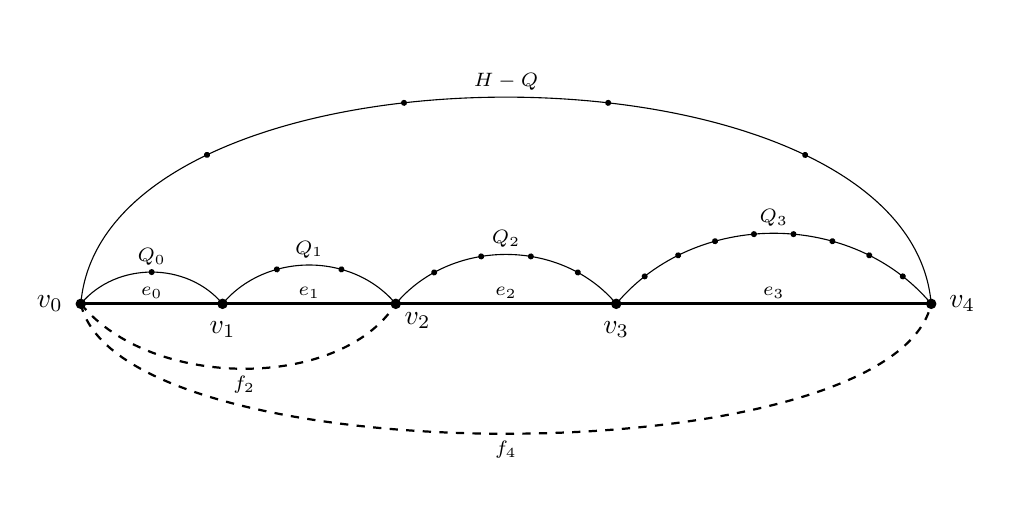
\begin{tikzpicture}[
  iv/.style 2 args={postaction={decorate,decoration={markings,
      mark=between positions #1 and #2 step #1 with {\fill (0,0) circle (1.1pt);}}}}]
  \coordinate (v0) at (0,0);
  \coordinate (v1) at (1.8,0);
  \coordinate (v2) at (4.0,0);
  \coordinate (v3) at (6.8,0);
  \coordinate (v4) at (10.8,0);
  \draw[iv={0.5}{0.51}]    (v0) to[bend left=50] node[pos=0.5,above=-1pt] {\scriptsize$Q_0$} (v1);
  \draw[iv={0.3333}{0.67}] (v1) to[bend left=50] node[pos=0.5,above=-1pt] {\scriptsize$Q_1$} (v2);
  \draw[iv={0.2}{0.81}]    (v2) to[bend left=50] node[pos=0.5,above=-1pt] {\scriptsize$Q_2$} (v3);
  \draw[iv={0.1111}{0.89}] (v3) to[bend left=50] node[pos=0.5,above=-1pt] {\scriptsize$Q_3$} (v4);
  \draw[iv={0.2}{0.81}]    (v0) .. controls (0.3,3.5) and (10.5,3.5) .. node[pos=0.5,above=-1pt] {\scriptsize$H-Q$} (v4);
  \foreach \a/\b/\i in {v0/v1/0,v1/v2/1,v2/v3/2,v3/v4/3}
    \draw[very thick] (\a) -- node[pos=0.5,above=-2pt] {\scriptsize$e_{\i}$} (\b);
  \draw[thick,dashed] (v0) .. controls (0.9,-1.1) and (3.3,-1.1) .. node[pos=0.5,below=-1pt] {\scriptsize$f_2$} (v2);
  \draw[thick,dashed] (v0) .. controls (0.5,-2.2) and (10.3,-2.2) .. node[pos=0.5,below=-1pt] {\scriptsize$f_4$} (v4);
  \foreach \p in {v0,v1,v2,v3,v4} \fill (\p) circle (1.9pt);
  \node[left=3pt] at (v0) {$v_0$};
  \node[below=3pt] at (v1) {$v_1$};
  \node[anchor=north west,inner sep=3pt] at (v2) {$v_2$};
  \node[below=3pt] at (v3) {$v_3$};
  \node[right=3pt] at (v4) {$v_4$};
\end{tikzpicture}
\caption{The construction for $n=24$, where $k=4$. The segments $Q_0,\dots,Q_3$ of the outer cycle
$H$ have $2,3,5,9$ edges and are doubled by the chords $e_0,\dots,e_3$. The chord $f_4$ gives the
cycle lengths $5,\dots,20$, the rest $H-Q$ of the outer cycle gives $9,\dots,24$, and $f_2$ gives
$3,\dots,6$.}
\label{fig:necklace}
\end{figure}

\section{The number of cycles}\label{sec:cycles}

For the lower bound $\psi(r)>2^{r-1}$, let $k=r-1$ and replace every edge of a cycle of length $k$
by a four-cycle in which the two ends of the edge are opposite vertices. The resulting graph has
rank $k+1=r$, and its cycles are the $k$ four-cycles and the $2^{k}$ cycles that use one half of
each four-cycle; so $\psi(r)\ge2^{r-1}+r-1$. Horak and Kim~\cite{HK} obtained
$\psi(r)\ge2^{r-1}+c\,r\,2^{r/2}$.

\begin{proof}[Proof of Theorem~\ref{thm:cycles}]
Let $r$ be large and let $G_0$ be a graph of rank $r$ with $\psi(r)$ cycles. The
following operations change neither the rank nor the number of cycles: identifying a vertex of one
component with a vertex of another; deleting a vertex of degree at most one; replacing a vertex of
degree two and its two edges by a single edge. The last operation may create loops and parallel
edges; a loop counts as a cycle of length one and two parallel edges form a cycle of length two.
Applying the operations as long as possible, we obtain a connected multigraph $K$ of rank $r$ with
$\psi(r)$ cycles and minimum degree at least $3$, and hence with at most $2r-2$ vertices.

\emph{Claim.} If $K'$ is obtained from $K$ by deleting $j$ edges and $K'$ contains a cycle, then
$K'$ contains a cycle with at most $2\log r+2j+4$ edges.

Indeed, call $\sum_v\max(0,3-\deg v)$ the deficit of a multigraph; the deficit of $K'$ is at most
$2j$. Deleting a vertex of degree at most one does not increase the deficit, so after deleting such
vertices as long as possible we are left with a multigraph $K_1$ of minimum degree at least two with
at most $2j$ vertices of degree two. If a component of $K_1$ is a cycle, that cycle has at most $2j$
edges. Otherwise replace each vertex of degree two by an edge; the result $K_2$ has minimum degree at
least $3$ and at most $2r-2$ vertices. Let $d=\lceil\log(2r)\rceil$. If $K_2$ had no cycle with at
most $2d$ edges, the vertices at distance at most $d$ from a given vertex would be distinct, and
there would be at least $3\cdot2^{d}-2>2r$ of them. A cycle of $K_2$ with at most $2d$ edges comes
from a cycle of $K_1$ with at most $2d+2j\le2\log r+2j+4$ edges. This proves the claim.

Now let $t=\lfloor(\log r)/100\rfloor$. For $i=1,\dots,t$ let $C_i$ be a shortest cycle of
$K-\{e_1,\dots,e_{i-1}\}$, which has positive rank, and let $e_i$ be one of its edges. By the claim, $|C_i|\le3\log r$. The
cycles $C_1,\dots,C_t$ are linearly independent in $\Z(K)$, because $e_i\in C_i$ and $e_i\notin C_j$
for $j>i$.

Let $G$ be the graph obtained from $K$ by subdividing every edge twice. It is simple and connected,
has rank $r$, and has $\psi(r)$ cycles. Let $W\subseteq G$ be the union of the cycles that correspond
to $C_1,\dots,C_t$. Then $\beta(W)\ge t$, and $W$ has at most $t\le(\log r)/100$ components and at
most $9t\log r\le\sqrt r$ edges. By Lemma~\ref{lem:count}(a) and Theorem~\ref{thm:forest},
\[
  \psi(r)\;\le\;2^{r}\bigl(p(G,W)+2^{-t}\bigr)\;\le\;2^{r}\Bigl(\frac12+\frac{20}{\lgk3r}+2r^{-1/100}\Bigr)
  \;\le\;\Bigl(\frac12+\frac{21}{\lgk3r}\Bigr)2^{r}.\qedhere
\]
\end{proof}

\begin{remark}\label{rem:asymptotic}
Theorem~\ref{thm:cycles} is purely asymptotic. Its bound is below the trivial bound $2^{r}$ only
when $\lgk3r>42$, that is, for $r>2^{2^{2^{42}}}$; it is below the bound $\frac{15}{16}2^{r}$
of~\cite{AT} only when $\lgk3r>48$; and the threshold $r_0$ of Theorem~\ref{thm:forest} is not
explicit. So for graphs of any moderate rank $\frac{15}{16}2^{r}$ remains the best bound known, and
the theorem says nothing about the second-order term of $\psi(r)$ (see
Section~\ref{sec:problems}).
\end{remark}


\section{Proof of the forest estimate}\label{sec:forest}

In this section graphs may have loops and parallel edges. A loop adds two to the degree of its vertex
and is a cycle of length one; two parallel edges form a cycle of length two. For a set $A$ of
vertices of $G$ we write $G[A]$ for the induced subgraph, $G-A$ for $G[V(G)\sm A]$, and $\delta A$
for the set of edges with exactly one end in $A$. A \emph{region} is a nonempty set $A$ such that
$G[A]$ is connected; it is \emph{cyclic} if $G[A]$ contains a cycle. As before $\xi$ is uniform on
$\Z(G)$, and $\cO_A$ denotes the event $\xi\cap\delta A=\emptyset$.

\subsection{Two cuts share at most one bit}

\begin{lemma}\label{lem:second}
Let $Z\ge0$ be a random variable with $\mu=\EE Z>0$ and $\EE Z^{2}\le2\mu^{2}+K\mu$. Then
$\PP(Z=0)\le\half+K/(4\mu)$.
\end{lemma}

\begin{proof}
By the Cauchy--Schwarz inequality $\mu^{2}\le\EE Z^{2}\cdot\PP(Z>0)$, so
$\PP(Z=0)\le1-\mu/(2\mu+K)\le\half+K/(4\mu)$.
\end{proof}

For disjoint regions $A,B$ of a connected graph $G$ let $\ell(A,B)$ be the number of \emph{links}
between them: the edges with one end in $A$ and the other in $B$, and the components of
$G-(A\cup B)$ that are joined by an edge to $A$ and by an edge to $B$.

\begin{lemma}[Link formula]\label{lem:link}
Let $A$ and $B$ be disjoint regions of a connected graph $G$. Then
$\PP(\cO_A)=2^{\comp(G-A)-|\delta A|}\ge2^{-|\delta A|}$ and
\[
  \PP(\cO_A\cap\cO_B)=2^{\ell(A,B)-1}\,\PP(\cO_A)\,\PP(\cO_B).
\]
Conditionally on $\cO_A$, the set $\xi\cap E(G[A])$ is uniform on $\Z(G[A])$; conditionally on
$\cO_A\cap\cO_B$, the sets $\xi\cap E(G[A])$ and $\xi\cap E(G[B])$ are independent and uniform on
$\Z(G[A])$ and $\Z(G[B])$.
\end{lemma}

\begin{proof}
The even subgraphs that avoid $\delta A$ are the sums of an even subgraph of $G[A]$ and an even
subgraph of $G-A$. So $\PP(\cO_A)=2^{\beta(G[A])+\beta(G-A)-\beta(G)}$, and counting edges and
vertices shows that the exponent is $\comp(G-A)-|\delta A|$. In the same way
\[
  \PP(\cO_A\cap\cO_B)=2^{\beta(G[A])+\beta(G[B])+\beta(G-A-B)-\beta(G)}
     =2^{\comp(G-A-B)+1-|\delta A|-|\delta B|+e(A,B)},
\]
where $e(A,B)$ is the number of edges between $A$ and $B$. Let $a$, $b$ and $k$ be the numbers of
components of $G-A-B$ that are joined to $A$ only, to $B$ only, and to both. Then
$\comp(G-A-B)=a+b+k$, while $\comp(G-A)=a+1$ and $\comp(G-B)=b+1$, and the formula follows since
$\ell(A,B)=k+e(A,B)$. The conditional laws are read off from the two direct sum decompositions.
\end{proof}

So two cut events are independent when there is one link, correlated by a factor of exactly two
when there are two, and more strongly correlated only for pairs with at least three links. The next
lemma says that such pairs are rare.

\begin{lemma}[Exceptional partners]\label{lem:exc}
Let $A$ be a region of a connected graph $G$, and let $B_1,\dots,B_k$ be pairwise disjoint regions,
disjoint from $A$, with $\ell(A,B_i)\ge3$ for all $i$. Then $k\le|\delta A|$.
\end{lemma}

\begin{proof}
Contract $A$ to a vertex $a$ and each $B_i$ to a vertex $b_i$, and delete the loops that arise.
This changes neither $d=|\delta A|$ nor the numbers $\ell(A,B_i)$, because the sets $B_j$ with
$j\ne i$ are connected and are contracted inside components of $G-(A\cup B_i)$. Let $F$ be a spanning forest of
$G-a$, and for every edge $e=au$ at $a$ attach a new leaf $\tau_e$ to $u$. Call the resulting forest
$F^{+}$ and its $d$ new leaves \emph{terminals}.

Fix $i$. Every link between $a$ and $b_i$ yields a path of $F^{+}$ from $b_i$ to a terminal. For an
edge $e=ab_i$ it is the edge $b_i\tau_e$. For a component $D$ of $G-\{a,b_i\}$ joined to both, choose
an edge $e=au$ with $u\in D$ and take the path of $F^{+}$ from $b_i$ to $\tau_e$; after its first
vertex it stays in $D\cup\{\tau_e\}$. Paths that come from different links therefore start with
different edges at $b_i$, and the union of any two of them is a path between two terminals. Let
$F^{\circ}\subseteq F^{+}$ be the union of all paths between terminals. As $\ell(a,b_i)\ge3$, the
vertex $b_i$ has degree at least $3$ in $F^{\circ}$. All leaves of $F^{\circ}$ are terminals, and a
forest with at most $d$ leaves has at most $d-2$ vertices of degree at least $3$. Hence $k\le d-2$.
\end{proof}

\begin{lemma}[Many small cuts]\label{lem:smallcuts}
Let $A_1,\dots,A_k$ be pairwise disjoint cyclic regions of a connected graph $G$ with
$|\delta A_i|\le d$ for all $i$. Then
\[
  \PP\bigl(\xi\cap E(G[A_i])\text{ is a forest for every }i\bigr)\;\le\;\frac12+\frac{(d+1)\,2^{d-1}}{k}.
\]
\end{lemma}

\begin{proof}
Let $E_i$ be the event that $\cO_{A_i}$ holds and $\xi\cap E(G[A_i])\ne\emptyset$. On $E_i$ the set
$\xi\cap E(G[A_i])$ is a nonempty even subgraph, hence not a forest, so it suffices to bound
$\PP(Z=0)$ for $Z=\sum_i\mathbf{1}_{E_i}$. By Lemma~\ref{lem:link},
$p_i:=\PP(E_i)=\PP(\cO_{A_i})\bigl(1-2^{-\beta(G[A_i])}\bigr)\ge2^{-d-1}$ and
$\PP(E_i\cap E_j)=2^{\ell(A_i,A_j)-1}p_ip_j$ for $i\ne j$. If $\ell(A_i,A_j)\le2$ this is at most
$2p_ip_j$. Otherwise we use $\PP(E_i\cap E_j)\le p_i$; by Lemma~\ref{lem:exc} this happens for at
most $d$ indices $j$, for each $i$. Hence $\EE Z^{2}\le\mu+2\mu^{2}+d\mu$ with
$\mu=\EE Z\ge k\,2^{-d-1}$, and Lemma~\ref{lem:second} gives the claim.
\end{proof}

\subsection{Reduction to a subcubic graph}

\begin{lemma}\label{lem:reduce}
Let $G$ and $W$ be as in Theorem~\ref{thm:forest}, with $m=|E(W)|$ and $c=\comp(W)$. There are a
connected multigraph $\Gamma$ with $\beta(\Gamma)=r$ and all degrees at most $3$, and a set
$P\subseteq V(\Gamma)$, such that
\begin{enumerate}
\item[\textup{(i)}] every vertex outside $P$ has degree $3$, $|P|\le2m$, and $\Gamma[P]$ has at
most $c$ components;
\item[\textup{(ii)}] $p(G,W)\le\PP\bigl(\xi_\Gamma\cap E(\Gamma-P)\text{ is a forest}\bigr)$, where
$\xi_\Gamma$ is uniform on $\Z(\Gamma)$.
\end{enumerate}
In particular $2r-2\le|V(\Gamma)|\le2r+2m$.
\end{lemma}

\begin{proof}
\emph{Splitting.} Replace every vertex $v$ of degree $d\ge4$ by a path $v^{1}v^{2}\cdots v^{d-2}$
and distribute the $d$ edges at $v$ along it in some order: two to $v^{1}$, one to each of
$v^{2},\dots,v^{d-3}$, and two to $v^{d-2}$. If $v\in V(W)$, let the edges of $W$ at $v$ come first
in this order, so that they end in an initial segment $v^{1},\dots,v^{i}$ of the path with
$i<\deg_W(v)$. Let $G'$ be the new graph; its degrees are at most $3$. Let $P$ consist of these
initial segments and of the vertices of $W$ that were not split. Then $|P|\le\sum_v\deg_W(v)=2m$,
every edge of $W$ joins two vertices of $P$, and $G'[P]$ has at most $c$ components.

Contracting the new path edges maps $\Z(G')$ bijectively onto $\Z(G)$, so we may take
$\xi_G=\xi_{G'}\cap E(G)$. Every edge of $G'-P$ is a new path edge or an edge of $E(G)\sm E(W)$. If
$\xi_G\sm E(W)$ is a forest, then so is its union with the set of all new path edges, because
contracting these edges, which form a forest, gives back $\xi_G\sm E(W)$. Hence
$p(G,W)\le\PP\bigl(\xi_{G'}\cap E(G'-P)\text{ is a forest}\bigr)$.

\emph{Cleaning.} As long as possible, delete a vertex of degree one outside $P$, or replace a vertex
of degree two outside $P$ and its two edges by a single edge. An even subgraph avoids a pendant edge
and contains both or none of the two edges at a vertex of degree two, so these operations induce
bijections of the cycle spaces. Let $\Gamma$ be the final multigraph. Each edge of $\Gamma-P$ is a
path of $G'$ all of whose vertices lie outside $P$; so if $\xi_\Gamma$ contains a cycle of
$\Gamma-P$, then the corresponding $\xi_{G'}$ contains a cycle of $G'-P$. This proves~(ii).

Edges with both ends in $P$ are never removed, so the vertices of $P$ keep degree at least two, and
the number of components of the graph induced on $P$ does not increase. The vertices outside $P$ now
have degree exactly $3$. Finally $3|V(\Gamma)|-|P|\le2|E(\Gamma)|\le3|V(\Gamma)|$ and
$|E(\Gamma)|=|V(\Gamma)|+r-1$ give the bounds on $|V(\Gamma)|$.
\end{proof}

\subsection{Parameters, and removing the short cycles}

From now on $\Gamma$ and $P$ are as in Lemma~\ref{lem:reduce}, $\xi=\xi_\Gamma$, and $r$ is large.
All $o(\cdot)$ and $O(\cdot)$ refer to $r\to\infty$ and are uniform in $G$ and $W$. Put
\begin{gather*}
  x=\log r,\qquad y=\log x,\qquad z=\log y,\\
  D=\lfloor x/10\rfloor,\qquad L=\lfloor x\sqrt y\rfloor,\qquad
  s=\lfloor(D-1)/2\rfloor,\qquad\varepsilon=20/z .
\end{gather*}
Recall that $|P|\le2\sqrt r$ and $c\le x/100$. Let $\mathcal{F}$ be the event that
$\xi\cap E(\Gamma-P)$ is a forest. We assume that
\begin{equation}\label{eq:assume}
  \PP(\mathcal{F})>\tfrac12+\varepsilon
\end{equation}
and derive a contradiction; by Lemma~\ref{lem:reduce}(ii) this proves Theorem~\ref{thm:forest}.

Let $\mathcal{Q}$ be a maximal family of pairwise disjoint cycles of $\Gamma-P$ of length at most $D$,
loops and pairs of parallel edges included, and let $S$ be the union of their vertex sets. For
$Q\in\mathcal{Q}$ the set $V(Q)$ is a cyclic region of $\Gamma$ with $|\delta V(Q)|\le|Q|\le D$,
because its vertices have degree $3$. On $\mathcal{F}$ the set $\xi\cap E(\Gamma[V(Q)])$ is a forest
for every $Q$, so Lemma~\ref{lem:smallcuts} and~\eqref{eq:assume} give
$|\mathcal{Q}|<(D+1)2^{D-1}/\varepsilon\le\sqrt r$. Hence $|S|\le D\sqrt r$.

Let $J=\Gamma-(P\cup S)$. By the maximality of $\mathcal{Q}$, $J$ is a simple graph of girth greater
than $D$. It has $v=2r+O(\sqrt r\log r)$ vertices, each of degree $3$ in $\Gamma$, so its
\emph{deficit} satisfies
\begin{equation}\label{eq:deficit}
  d_J:=\sum_{u\in V(J)}\bigl(3-\deg_Ju\bigr)\;\le\;3\bigl(|P|+|S|\bigr)=O(\sqrt r\log r).
\end{equation}

\subsection{Cycles of moderate length}

A walk $u_0u_1\cdots u_\ell$ is \emph{non-backtracking} if $u_{i+1}\ne u_{i-1}$ for $0<i<\ell$. Let
$N_\ell(u,w)$ be the number of non-backtracking walks of length $\ell$ from $u$ to $w$ in $J$.

\begin{lemma}\label{lem:walks}
If $\ell>s$, then $N_\ell(u,w)\le3\cdot2^{\ell-s-1}$ for all $u,w$. Consequently, for every vertex
$u$ of $J$, the cycles $C$ of $J$ through $u$ with $|C|\le L$ satisfy $\sum_C2^{-|C|}\le L\,2^{-s}$.
\end{lemma}

\begin{proof}
There are at most $3\cdot2^{\ell-s-1}$ ways to choose the first $\ell-s$ steps. The last $s$ steps
form a non-backtracking walk of length $s$ between two given vertices. Such a walk is a path,
because $s$ is less than the girth, and there is at most one such path, because two of them would
give a cycle of length at most $2s<D$. For the second statement, a cycle of length $\ell$ through $u$
can be traversed from $u$ in two directions, so there are at most $\half N_\ell(u,u)$ of them, and
$\ell>D>s$.
\end{proof}

Let $B$ be the non-backtracking matrix of $J$. Its rows and columns are indexed by the directed
edges $(i\to j)$ of $J$, two for each edge, and the entry in row $(i\to j)$ and column $(j'\to k)$
is $1$ if $j'=j$ and $k\ne i$, and $0$ otherwise.

\begin{lemma}\label{lem:spectrum}
For every even $\ell\ge2$,
\[
  \tr B^{\ell}\;\ge\;\bigl(2-d_J/v\bigr)^{\ell}-3v\,2^{\ell/2}.
\]
\end{lemma}

\begin{proof}
Let $A$ be the adjacency matrix of $J$ and $\Delta$ the diagonal matrix of its degrees, and put
$M(\lambda)=\lambda^{2}I-\lambda A+\Delta-I$.

(1) \emph{If $M(\lambda)g=0$ for a real $\lambda>1$ and a vector $g\ne0$, then $\lambda$ is an
eigenvalue of $B$.} A direct computation shows that $f(i\to j)=\lambda g(j)-g(i)$ satisfies
$Bf=\lambda f$; and $f=0$ would give $g(i)=\lambda g(j)=\lambda^{2}g(i)$ along every edge, hence
$g=0$ (at an isolated vertex, $M(\lambda)g=0$ already says $(\lambda^{2}-1)g=0$).

(2) \emph{If $Bf=\lambda f$ with $f\ne0$ and $\lambda^{2}\ne1$, then $M(\lambda)g=0$ for
$g(j)=\sum_{k\sim j}f(j\to k)$, and $g\ne0$.} The eigenvalue equation at $(i\to j)$ and at
$(j\to i)$ reads $\lambda f(i\to j)=g(j)-f(j\to i)$ and $\lambda f(j\to i)=g(i)-f(i\to j)$.
Eliminating $f(j\to i)$ gives $(\lambda^{2}-1)f(i\to j)=\lambda g(j)-g(i)$, and summing this over
the neighbours $j$ of $i$ gives $M(\lambda)g=0$.

(3) \emph{$B$ has a real eigenvalue $\lambda_1\ge2-d_J/v$.} The matrix
$M(2)=2(\Delta-A)+(3I-\Delta)$ is positive semidefinite, while
$\mathbf{1}^{\!\top}M(\lambda)\mathbf{1}=(\lambda-1)(v\lambda-2v+d_J)$ vanishes at
$\lambda^{*}=2-d_J/v>1$. The smallest eigenvalue of the symmetric matrix $M(\lambda)$ is continuous
in $\lambda$, at most $0$ at $\lambda^{*}$ and at least $0$ at $2$. So $M(\lambda_1)$ is singular for
some $\lambda_1\in[\lambda^{*},2]$, and (1) applies.

(4) \emph{Every non-real eigenvalue $\lambda$ of $B$ satisfies $|\lambda|\le\sqrt2$.} With $g$ as
in~(2), $g^{*}M(\lambda)g=0$ is a quadratic equation $a\lambda^{2}-b\lambda+c'=0$ with real
coefficients $a=g^{*}g>0$, $b=g^{*}Ag$ and $c'=g^{*}(\Delta-I)g\le2a$. Its roots are $\lambda$ and
$\bar\lambda$, so $|\lambda|^{2}=c'/a\le2$.

Now $\tr B^{\ell}$ is the sum of the $\ell$th powers of the $2|E(J)|\le3v$ eigenvalues of $B$. For
even $\ell$ the real eigenvalues contribute nonnegative terms, one of which is at least
$(2-d_J/v)^{\ell}$, and the non-real ones contribute at least $-3v\,2^{\ell/2}$ in total.
\end{proof}

Facts (2) and (4) are part of the Ihara--Bass theory~\cite{Bass,KS}; the use of the test vector
$\mathbf{1}$ in~(3), which makes the argument work without any assumption of regularity or
expansion, is from~\cite{KNT}.

\begin{lemma}[Cycle weight]\label{lem:weight}
Let $\mathcal{C}$ be the set of cycles of $J$ of length at most $L$. Then
\[
  V:=\sum_{C\in\mathcal{C}}2^{-|C|}\;\ge\;\bigl(\tfrac18-o(1)\bigr)\ln y .
\]
\end{lemma}

\begin{proof}
$\tr B^{\ell}$ is the number of closed walks $u_0u_1\cdots u_\ell=u_0$ in $J$ with
$u_{i+1}\ne u_{i-1}$ for all $i$ modulo $\ell$. A cycle of length $\ell$ gives $2\ell$ of them; let
$n_\ell$ be the number of the others. Then
\[
  T:=\sum_{\ell\le L}\frac{\tr B^{\ell}}{2\ell\,2^{\ell}}=V+\sum_{\ell\le L}\frac{n_\ell}{2\ell\,2^{\ell}} .
\]
Consider a walk counted by $n_\ell$, and let $j$ be the least index with
$u_j\in\{u_0,\dots,u_{j-1}\}$, say $u_j=u_i$. Then $j<\ell$, the walk $Q=u_iu_{i+1}\cdots u_j$ is a
cycle, of length $q$ say, and $u_ju_{j+1}\cdots u_\ell u_1\cdots u_i$ is a non-backtracking closed
walk of length $\ell-q>0$ from $u_i$ to itself. It contains a cycle, so $\ell-q>D>s$. The original
walk is determined by $Q$, by the vertex $u_i$ and a direction on $Q$ ($2q$ choices), by the
complementary walk (at most $3\cdot2^{\ell-q-s-1}$ choices, by Lemma~\ref{lem:walks}), and by the
position of $u_0$ on the latter (at most $\ell$ choices). Hence
\[
  \sum_{\ell\le L}\frac{n_\ell}{2\ell\,2^{\ell}}
  \;\le\;\sum_{\ell\le L}\ \sum_{Q\in\mathcal{C}}\tfrac32\,|Q|\,2^{-|Q|-s}
  \;\le\;\tfrac32\,L^{2}\,2^{-s}\,V=o(V),
\]
because $2^{-s}\le8\,r^{-1/20}$ and $L^{2}\le x^{2}y$.

On the other hand, for even $\ell$ with $6x\le\ell\le L$, Lemma~\ref{lem:spectrum}
and~\eqref{eq:deficit} give
\[
  2^{-\ell}\tr B^{\ell}\;\ge\;\Bigl(1-\frac{d_J}{2v}\Bigr)^{\ell}-3v\,2^{-\ell/2}
  \;\ge\;1-\frac{L\,d_J}{2v}-3v\,r^{-3}=1-o(1).
\]
All terms of $T$ are nonnegative, so $T\ge(1-o(1))\sum1/(2\ell)$ over the even $\ell$ in $[6x,L]$,
and this sum is $(\frac14-o(1))\ln(L/6x)=(\frac18-o(1))\ln y$. Therefore
$V=(1-o(1))T\ge(\frac18-o(1))\ln y$.
\end{proof}

\subsection{The second moment}

For $C\in\mathcal{C}$ let $I_C$ be the event that $C$ is a component of $\xi$. As the vertices of
$C$ have degree $3$ in $\Gamma$, this is the event $E(C)\subseteq\xi$; it is also the event that
$\cO_{V(C)}$ holds and $\xi\cap E(\Gamma[V(C)])=E(C)$. Put
\[
  a_C=2^{-|C|},\qquad p_C=\PP(I_C),\qquad X_C=\frac{a_C}{p_C}\,\mathbf{1}_{I_C},\qquad
  Z=\sum_{C\in\mathcal{C}}X_C .
\]
The event $I_C$ is given by $|C|$ linear conditions on $\xi\in\Z(\Gamma)$, which are satisfied by
$\xi=C$; so $p_C\ge a_C$. Hence $0\le X_C\le1$, $\EE X_C=a_C$ and $\mu:=\EE Z=V$. On $\mathcal{F}$
no cycle of $J\subseteq\Gamma-P$ is contained in $\xi$, so $Z=0$, and by~\eqref{eq:assume}
\begin{equation}\label{eq:Zzero}
  \PP(Z=0)>\tfrac12+\varepsilon .
\end{equation}

Let $C\ne C'$ be in $\mathcal{C}$. If they share a vertex, then $I_C\cap I_{C'}=\emptyset$. If they
are disjoint, Lemma~\ref{lem:link}, applied to the regions $V(C)$ and $V(C')$ of $\Gamma$, gives
$\PP(I_C\cap I_{C'})=2^{\ell(C,C')-1}p_Cp_{C'}$ and therefore
\begin{equation}\label{eq:pair}
  \EE(X_CX_{C'})=a_Ca_{C'}\,2^{\ell(C,C')-1},
\end{equation}
where $\ell(C,C')$ is the number of links between $V(C)$ and $V(C')$ in $\Gamma$.

\begin{lemma}[Few links]\label{lem:links}
$\ell(C,C')\le c+o(x)$ for all disjoint $C,C'\in\mathcal{C}$.
\end{lemma}

\begin{proof}
Let $U=V(C)\cup V(C')$. Every vertex of $U$ lies on exactly one edge outside its own cycle, so at
most $2L$ edges leave $U$. At most $c$ components of $\Gamma-U$ meet $P$, because $P\cap U=\emptyset$
and so each component of $\Gamma[P]$ lies in one of them. Let $Y$ run over the other components and
let $d_Y$ be the number of edges between $Y$ and $U$; then $\sum_Yd_Y\le2L$. Put
$t_0=\lfloor y/2\rfloor$.

\emph{Large cuts.} At most $2L/t_0$ components have $d_Y>t_0$.

\emph{Small cuts, cyclic.} The components $Y$ with $d_Y\le t_0$ that are cyclic are pairwise
disjoint cyclic regions inside $\Gamma-P$ with $|\delta Y|\le t_0$. On $\mathcal{F}$ each
$\xi\cap E(\Gamma[Y])$ is a forest, so by Lemma~\ref{lem:smallcuts} and~\eqref{eq:assume} there are
fewer than $(t_0+1)2^{t_0-1}/\varepsilon$ of them.

\emph{Small cuts, trees.} Let $Y$ induce a tree, with $d_Y\le t_0$. No $Q\in\mathcal{Q}$ meets $Y$,
since $Q$ is a connected subgraph of $\Gamma-U$ and would lie in $Y$. Hence $Y\subseteq V(J)$. As
all degrees are $3$, we have $3|Y|=2(|Y|-1)+d_Y$, that is, $|Y|=d_Y-2$. So if $Y$ is joined to both
cycles, there is a path $R$ from $C$ to $C'$ through $Y$ with at most $t_0$ edges. For a link that
is an edge, let $R$ be that edge. The paths $R$ obtained in this way lie in $J$ and are pairwise
disjoint. Divide each of $C$ and $C'$ into at most $8L/D$ blocks of at most $D/4$ consecutive
vertices. If two of the paths had their ends in the same block of $C$ and in the same block of $C'$,
they would form, together with two arcs inside these blocks, a cycle of $J$ of length less than
$2t_0+D/2\le D$. So there are at most $(8L/D)^{2}$ such paths.

Altogether
\[
  \ell(C,C')\;\le\;c+\frac{2L}{t_0}+\frac{(t_0+1)2^{t_0-1}}{\varepsilon}+\Bigl(\frac{8L}{D}\Bigr)^{2}
  =c+O\Bigl(\frac{x}{\sqrt y}\Bigr)+O\bigl(yz\sqrt x\bigr)+O(y)=c+o(x).\qedhere
\]
\end{proof}

\begin{proof}[Proof of Theorem~\ref{thm:forest}]
Call a disjoint pair $C,C'\in\mathcal{C}$ \emph{exceptional} if $\ell(C,C')\ge3$. Fix $C$, and let
$\mathcal{E}$ be a maximal family of pairwise disjoint exceptional partners of $C$. By
Lemma~\ref{lem:exc}, $|\mathcal{E}|\le|\delta V(C)|\le L$, so the union $U_C$ of their vertex sets
has at most $L^{2}$ vertices, and every exceptional partner of $C$ meets $U_C$. By
Lemma~\ref{lem:walks}, the sum of $a_{C'}$ over all $C'\in\mathcal{C}$ that meet $U_C$ is at most
$L^{3}2^{-s}$. With~\eqref{eq:pair} and Lemma~\ref{lem:links},
\[
  \sum_{C'\ \mathrm{exceptional}}\EE(X_CX_{C'})\;\le\;a_C\,2^{c+o(x)}L^{3}\,2^{-s}
  =a_C\,2^{\,c-x/20+o(x)}=o(a_C),
\]
because $c\le x/100$. For the other disjoint pairs $\EE(X_CX_{C'})\le2a_Ca_{C'}$, intersecting pairs
contribute nothing, and $\EE X_C^{2}\le\EE X_C=a_C$. Summing over $C$ we get
$\EE Z^{2}\le2\mu^{2}+(1+o(1))\mu$. By Lemmas~\ref{lem:second} and~\ref{lem:weight},
\[
  \PP(Z=0)\;\le\;\frac12+\frac{1+o(1)}{4\mu}\;\le\;\frac12+\frac{2+o(1)}{\ln y}\;<\;\frac12+\frac{20}{z}
\]
for large $r$, since $\ln y=z\ln2$. This contradicts~\eqref{eq:Zzero}.
\end{proof}

\begin{remark}\label{rem:range}
The assumption $|E(W)|\le\sqrt r$ entered only through $|P|\le2\sqrt r$ in~\eqref{eq:deficit}, where
all that is needed is $L\,d_J=o(v)$; the proof therefore works unchanged for
$|E(W)|\le r/\log^{2}r$. Similarly the constant $20$ can be replaced by any constant larger than
$2/\ln2$. We have kept the statement of~\cite{KNT}, which is the one that has been formalised.
\end{remark}

\section{Exact and nearly exact counting}\label{sec:exact}

By Lemma~\ref{lem:count} the cycles of $G$ have at most $2^{r-t}(pm+1-p)$ lengths, and
Theorem~\ref{thm:forest} says that $p\le\half+o(1)$ when $r$ is large. Here we look at the other end
of the scale. When is nothing lost, and what do graphs look like that lose little?

\subsection{Two terminals}

\begin{proposition}\label{prop:terminal}
Let $N$ be a connected graph and let $s\ne t$ be two of its vertices. Then $N$ has at most
$2^{\beta(N)}$ paths from $s$ to $t$. If it has exactly $2^{\beta(N)}$, then $N-E(A)$ is a forest
for every path $A$ from $s$ to $t$, and every such path has at least $\beta(N)$ edges.
\end{proposition}

\begin{proof}
A path from $s$ to $t$ is an $\{s,t\}$-join, and the joins form a coset of $\Z(N)$, so there are
$2^{\beta(N)}$ of them. Suppose that all joins are paths, and let $A$ be one of them. If $N-E(A)$
contained a cycle $C$, then $A\cup C=A+C$ would be a join that is not a path. So $N-E(A)$ is a
forest, and since deleting an edge lowers the cycle rank by at most one, $\beta(N)\le|A|$.
\end{proof}

Equivalently, an edge $f$ of a graph $G$ lies on at most $2^{\beta(G)-1}$ cycles, and if it lies on
that many, then each of them has at least $\beta(G)$ edges. Equality in
Proposition~\ref{prop:terminal} holds for the necklace $N_j$ of Section~\ref{sec:upper} between
$v_0$ and $v_j$, for $K_4$ minus an edge between its two vertices of degree two, and for $K_{3,3}$
minus an edge between the ends of the deleted edge.

This is the reason for the shape of the construction. The necklace $N_k$ turns $k$ units of rank
into $2^{k}$ path lengths, the most that $k$ units can give. But by
Proposition~\ref{prop:terminal} no gadget that does this has a path with fewer than $k$ edges
between its terminals. So the cycles through $N_k$ have length greater than $k$, and the lengths
$3,\dots,k$ have to be produced elsewhere: by a necklace with about $\log k$ beads, whose own short
lengths require a third one, and so on. Relative to each necklace $N_j$ that is closed by a chord $f_j$,
taken together with $f_j$ and the chords of the smaller necklaces, the rest of the graph is attached
at the two vertices $v_0$ and $v_j$ only, so that half of the words cannot be used
(Remark~\ref{rem:twoports}). These $\lgs k$ halvings are the term
$\lgs n$ of Theorem~\ref{thm:main}.

\subsection{No waste}

Call a word \emph{wasted} if it is not the outside part of any cycle. In Lemma~\ref{lem:count}
nothing is lost only if no word is wasted, and this cannot go on for long.

\begin{proposition}\label{prop:nowaste}
Let $G$ be a connected graph and let $W\subseteq G$ be a subgraph that contains a cycle. Suppose
that every coset of $\Z(W)$ in $\Z(G)$ contains a cycle. Then every nonempty even subgraph of
$G-E(W)$ is a cycle, and
\[
  \beta(G)-\beta(W)\;\le\;|V(W)|+3 .
\]
\end{proposition}

\begin{proof}
Let $z$ be a nonempty even subgraph of $G-E(W)$. All members of the coset $z+\Z(W)$ contain $z$, one
of them is a cycle, and a cycle that contains a nonempty even subgraph is equal to it. So $z$ is a
cycle. In particular the graph $G'=G-E(W)$, on the vertex set $V(G)$, has no two edge-disjoint
cycles, and by Lemma~\ref{lem:EP} below $|E(G')|\le|V(G)|+3$. Since $\beta(G)=|E(G)|-|V(G)|+1$ and
$\beta(W)\ge|E(W)|-|V(W)|+1$, we get $\beta(G)-\beta(W)\le|E(G')|-|V(G)|+|V(W)|\le|V(W)|+3$.
\end{proof}

\begin{lemma}[Erd\H{o}s and P\'osa~\cite{EP}]\label{lem:EP}
A multigraph with $n$ vertices and at least $n+4$ edges contains two edge-disjoint cycles.
\end{lemma}

\begin{proof}
We include the short proof. Let $H$ be a counterexample with $|V(H)|+|E(H)|$ minimal, and let $n$
be its number of vertices. Then $H$ has exactly $n+4$ edges and no vertex of degree at most one. It
has no vertex of degree two either: such a vertex could be replaced, together with its two edges, by
a single edge, or it carries a loop, and the rest of $H$ contains a second cycle. So
$2(n+4)\ge3n$, that is, $n\le8$. Let $C$ be a shortest cycle of $H$. Since $H-E(C)$ is a forest,
$n+4-|C|\le n-1$, so $|C|\ge5$. Thus $H$ is a simple graph of minimum degree at least $3$ and girth
at least $5$, and such a graph has at least $1+3+6=10$ vertices, a contradiction.
\end{proof}

The first conclusion of Proposition~\ref{prop:nowaste} is the graphic case of the fact that a binary
code in which every nonzero word is minimal is intersecting~\cite[\S2]{AACST}. The second is sharp up
to the additive constant. If $W$ is a cycle $w_1\cdots w_m$ and $G$ consists of $W$ and a path of
length two from $w_i$ to $w_{i+1}$ for every $i$ modulo $m$, then no word is wasted and
$\beta(G)-\beta(W)=|V(W)|$. If $G$ is $K_5$ minus an edge and $W$ is the triangle on its three
vertices of degree four, then no word is wasted and $\beta(G)-\beta(W)=|V(W)|+1$. An exhaustive
search found nothing better for a triangle $W$ in graphs with at most eight vertices.

So the trivial bound of $m\,2^{r-t}$ cycle lengths can be exact for at most $m+3$ ranks beyond
$W$, while by Theorem~\ref{thm:forest} it is off by a factor of almost two as soon as $r\ge m^{2}$,
for large $m$ and $W$ as in that theorem.

\subsection{A defect budget}

The last statement of this section is a stability version of the same picture: a graph that comes
close to the trivial bound must be built, at almost every step, the way the necklace is built.

Let $G$ contain a cycle of each length $3,\dots,L$, and let $\Theta=(L-2)\,2^{-\beta(G)}$. A
\emph{greedy sequence} is a sequence of subgraphs $W_1\subset W_2\subset\dots\subset W_Q$ of $G$ in
which $W_1$ is a triangle, $W_{q+1}=W_q\cup C_q$ for a cycle $C_q$ of $G$ whose length $\ell_q$ is
the least integer $\ge3$ that is not the length of a cycle of $W_q$, and $W_Q$ is the first term
that contains cycles of all lengths $3,\dots,L$. Write $m_q=|E(W_q)|$ and $t_q=\beta(W_q)$, and let
\[
  \rho_q=\frac{m_q+2}{2^{t_q}},\qquad
  \kappa_q=1-\frac{m_{q+1}-m_q}{m_q+2},\qquad
  j_q=t_{q+1}-t_q-1 .
\]

\begin{proposition}[Defect budget]\label{prop:defect}
For every greedy sequence:
\begin{enumerate}
\item[\textup{(i)}] $0<\kappa_q<1$, $j_q\ge0$ and $\rho_{q+1}=(1-\half\kappa_q)\,2^{-j_q}\rho_q$ for
$1\le q<Q$;
\item[\textup{(ii)}] $\Theta<\rho_q$ for all $q$, and therefore
$\sum_{q=a}^{Q-1}\bigl(\half\kappa_q+j_q\ln2\bigr)<\ln(\rho_a/\Theta)$ for every $a$;
\item[\textup{(iii)}] if $j_q=0$ and $\kappa_q\le\eta$, then $C_q$ has at least $(1-\eta)(m_q+2)$
edges outside $W_q$ and fewer than $\eta(m_q+2)$ edges in $W_q$, and $W_q$ has cycles of at least
$(1-\eta)(m_q+2)-3$ different lengths.
\end{enumerate}
\end{proposition}

\begin{proof}
(i) Let $P_q=E(C_q)\sm E(W_q)$, so that $|P_q|=m_{q+1}-m_q\ge1$. The graph $W_q$ has cycles of all
lengths $3,\dots,\ell_q-1$ and no cycle longer than $m_q$. Hence $|P_q|\le\ell_q\le m_q+1$ and
$0<\kappa_q<1$. Also $j_q\ge0$, because $C_q\in\Z(W_{q+1})\sm\Z(W_q)$, and the identity restates
$m_{q+1}+2=(2-\kappa_q)(m_q+2)$.

(ii) By Lemma~\ref{lem:count}(b) with $W=W_q$ and $p\le1$, the cycles of $G$ have at most
$m_q2^{\beta(G)-t_q}$ lengths, so $\Theta\le m_q2^{-t_q}<\rho_q$. By~(i),
$\rho_Q\le\rho_a\exp\bigl(-\sum_{q=a}^{Q-1}(\half\kappa_q+j_q\ln2)\bigr)$.

(iii) Here $|P_q|=(1-\kappa_q)(m_q+2)$, the number of edges of $C_q$ in $W_q$ is
$\ell_q-|P_q|\le m_q+1-|P_q|$, and $W_q$ has cycles of at least $\ell_q-3\ge|P_q|-3$ lengths.
\end{proof}

Call a step \emph{perfect} if $j_q=0$ and $\kappa_q\le\eta$. By~(ii), if $G$ comes within a factor
$K$ of the trivial bound $\Theta<\rho_a$ relative to $W_a$, then all but $(2/\eta)\ln K$ of the
steps after $W_a$ are perfect. By~(iii), a perfect step roughly doubles the graph by a new cycle
that closes through a part of $W_q$ of relative size less than $\eta$, at a moment when almost every
integer up to $m_q$ is the length of a cycle of $W_q$; and if $W_q$ is connected, $j_q=0$ means that
the new edges form a single path or cycle that meets $W_q$ in at most two vertices. These are the
features of a bead of the necklace. In this coarse sense the shape of the construction is forced
between any two halvings, and Theorem~\ref{thm:forest} forces the halvings.

\section{Problems}\label{sec:problems}

\paragraph{Error terms.}
By Remark~\ref{rem:twoports} the left side of~\eqref{eq:forest} can be as large as
$\half+2^{1-r}$, and Horak and Kim~\cite{HK} proved that $\psi(r)\ge2^{r-1}+c\,r\,2^{r/2}$ for some
$c>0$. The upper bounds of Theorems~\ref{thm:forest} and~\ref{thm:cycles} are very far from this. In
the proof, the gain $\mu$ comes from cycles with between $6\log r$ and $\log r\sqrt{\log\log r}$
edges. Each length $\ell$ contributes about $1/(2\ell)$, and the upper end of the range is dictated
by Lemma~\ref{lem:links}; so $\mu$ is only of order $\lgk3r$.

\begin{problem}
Is the error term in~\eqref{eq:forest} at most $r^{-c}$ for some $c>0$? Is
$\psi(r)\le2^{r-1}+2^{(1-c)r}$?
\end{problem}

\paragraph{Between exactness and the forest estimate.}
Proposition~\ref{prop:nowaste} and Theorem~\ref{thm:forest} are an exact and an asymptotic statement
about the same thing: no word is wasted for at most $|V(W)|+3$ ranks beyond $W$, and about half
of the words fail to be forests once $r\ge|E(W)|^{2}$, or already once $r\ge|E(W)|\log^{2}r$ by
Remark~\ref{rem:range}. We do not know a proof of the factor $\half$ that
avoids the second moment computation of Section~\ref{sec:forest}, except in special situations such
as Remark~\ref{rem:twoports}. A robust form of Proposition~\ref{prop:terminal} would be a step in
that direction.

\begin{problem}
Let $\varepsilon>0$. If a connected graph $N$ has at least $(\half+\varepsilon)2^{\beta(N)}$ paths
between two vertices $s$ and $t$, must each of these paths have at least $c(\varepsilon)\beta(N)$
edges?
\end{problem}

\begin{problem}
Can the constant $3$ in Proposition~\ref{prop:nowaste} be replaced by $1$?
\end{problem}

\begin{thebibliography}{99}\small

\bibitem{AACST} A.~Alahmadi, R.~E.~L.~Aldred, R.~dela~Cruz, P.~Sol\'e and C.~Thomassen, The maximum
number of minimal codewords in long codes, \emph{Discrete Appl.\ Math.}\ \textbf{161} (2013),
424--429. arXiv:1201.6043.

\bibitem{AT} R.~E.~L.~Aldred and C.~Thomassen, On the maximum number of cycles in a planar graph,
\emph{J.~Graph Theory} \textbf{57} (2008), 255--264.

\bibitem{Bass} H.~Bass, The Ihara--Selberg zeta function of a tree lattice, \emph{Internat.\
J.~Math.}\ \textbf{3} (1992), 717--797.

\bibitem{Bloom} T.~F.~Bloom, Erd\H{o}s Problem \#1016, \url{https://www.erdosproblems.com/1016},
accessed November 2026.

\bibitem{Bondy} J.~A.~Bondy, Pancyclic graphs~I, \emph{J.~Combin.\ Theory Ser.~B} \textbf{11}
(1971), 80--84.

\bibitem{ES} R.~C.~Entringer and P.~J.~Slater, On the maximum number of cycles in a graph,
\emph{Ars Combin.}\ \textbf{11} (1981), 289--294.

\bibitem{EP} P.~Erd\H{o}s and L.~P\'osa, On the maximal number of disjoint circuits of a graph,
\emph{Publ.\ Math.\ Debrecen} \textbf{9} (1962), 3--12.

\bibitem{GKW} J.~C.~George, A.~Khodkar and W.~D.~Wallis, \emph{Pancyclic and Bipancyclic Graphs},
SpringerBriefs in Mathematics, Springer, 2016.

\bibitem{Griffin} S.~Griffin, Minimal pancyclicity, arXiv:1312.0274 (2013).

\bibitem{HK} P.~Horak and D.~Kim, Connected cubic graphs with the maximum number of perfect
matchings, \emph{J.~Graph Theory} \textbf{99} (2022), 671--690. arXiv:2006.13459.

\bibitem{KNT} KNT, The minimum number of edges in a pancyclic graph, manuscript, September 2026,
\url{https://jehlp.net/erdos1016/}; Lean~4 formalisation at
\url{https://github.com/JWKNT/erdos1016}.

\bibitem{KS} M.~Kotani and T.~Sunada, Zeta functions of finite graphs, \emph{J.~Math.\ Sci.\ Univ.\
Tokyo} \textbf{7} (2000), 7--25.

\end{thebibliography}

\end{document}
